\documentclass[
11pt,%
tightenlines,%
twoside,%
onecolumn,%
nofloats,%
nobibnotes,%
nofootinbib,%
superscriptaddress,%
noshowpacs,%
centertags]%
{revtex4}
\usepackage{ljm}
\usepackage{listings}

\lstset{
language=C++,
basewidth=0.5em,
xleftmargin=45pt,
xrightmargin=45pt,
basicstyle=\small\ttfamily,
keywordstyle=\bfseries\underbar,
numbers=left,
numberstyle=\tiny,
stepnumber=1,
numbersep=10pt,
showspaces=false,
showstringspaces=false,
showtabs=false,
frame=trBL,
tabsize=2,
captionpos=t,
breaklines=true,
breakatwhitespace=false,
escapeinside={\%*}{*)}
}

\begin{document}

\titlerunning{Process Mining}
\authorrunning{Savin et al.}

\title{Process Mining: Realization and Optimization of Process Discovery Algorithm}

\author{\firstname{G.~I.}~\surname{Savin}}
\email[E-mail: ]{savin@jscc.ru}
\affiliation{Joint Supercomputer Center of the Russian Academy of Sciences -- branch of Scientific Research Institute of System Analysis of the Russian Academy of Sciences, Leninsky prospect 32a, Moscow, 119334, Russia}

\author{\firstname{A.~D.}~\surname{Chopornyak}}
\email[E-mail: ]{chopor@jscc.ru}
\affiliation{Joint Supercomputer Center of the Russian Academy of Sciences -- branch of Scientific Research Institute of System Analysis of the Russian Academy of Sciences, Leninsky prospect 32a, Moscow, 119334, Russia}

\author{\firstname{A.~A.}~\surname{Rybakov}}
\email[E-mail: ]{rybakov.aax@gmail.com}
\affiliation{Joint Supercomputer Center of the Russian Academy of Sciences -- branch of Scientific Research Institute of System Analysis of the Russian Academy of Sciences, Leninsky prospect 32a, Moscow, 119334, Russia}

\author{\firstname{S.~S.}~\surname{Shumilin}}
\email[E-mail: ]{shumilin@jscc.com}
\affiliation{Joint Supercomputer Center of the Russian Academy of Sciences -- branch of Scientific Research Institute of System Analysis of the Russian Academy of Sciences, Leninsky prospect 32a, Moscow, 119334, Russia}

\firstcollaboration{(Submitted by S.~S.~Submitter)}

\received{May 01, 2020}

\begin{abstract}
Abstract.
\end{abstract}

\subclass{} % Enter 2010 Mathematics Subject Classification.

\keywords{Keyword1, keyword2.}

\maketitle

\section{Introduction}

Process mining представляет собой совокупность подходов и методов по извлечению относящейся к процессам достоверной информации из данных, собранных в журналах событий.
Process mining является дополнением к технологии управления бизнес-процессами (Business Process Management, BPM), которая в свою очередь является расширением технологии управления рабочими процессами (Workflow Management, WFM).
Технология WFM исторически была направлена прежде всего на автоматизацию бизнес-процессов с механической точки зрения, тогда как с применением подходов BPM уделяется особое внимание другим аспектам, в которых могут быть скрыты узкие места (человеческий фактор, особенности организации, нечеткие правила и другие).
В настоящее время большинство информационных систем по анализу процессов (Process-Aware Information System, PAIS) в составе серьезного программного обеспечения класса планирования ресурсов предприятия (Enterprise Resource Planning, ERP), кроме классических инструментов WFM включает расширения BPM и подходы process mining.
Однако зачастую данные системы так и остаются системами анализа и уведомления, оказываясь недостаточно интегрированными в цифровое пространство.
Наряду с термином PAIS для таких систем применяется также термин BPMS (BPM System) или просто PMS (Process Management System).

Любая система анализа процессов работает с моделью процесса, которая записывается с использованием одной или нескольких нотаций.
Эти нотации представляют сущность процесса и по сути являются макроописаниями ориентированных графов специального вида.
Основными объектами моделей процессов являются активности, состояния, переходы и подпроцессы.
Переходы между разными активностями, также называют зависимостями.
Совокупность зависимостей между активностями и дополнительные условия, накладываемые на модель процесса, порождают множество возможных последовательностей смены состояний, или множество сценариев протекания процесса.
В зависимости от детализации процессов могут применяться дополнительные атрибуты любых объектов модели процесса: привязки ко времени, продолжительность активностей, логика зависимостей, ресурсы и стратегии их использования, роли исполнителей активностей и многие другие.
Такое многообразие, возникающее при моделировании процессов, порождает огромное количество методов анализа процессов и протекания сценариев, и может служить источником полезных и не всегда очевидных знаний, используемых для оптимизации процессов.

Модели процессов, записанные с помощью формальной нотации, могут быть использованы для различных целей: обзор (при разработке модели команда рассматривает процесс с различных точек зрения и может детально остановиться на отдельных ее локальных особенностях), обсуждение (формальная запись модели процесса с конкретных точек зрения делает возможным проведения дискуссии между всеми стейкхолдерами, участвующими в разработке модели), документация (формальная запись модели допускает даже автоматическое создание документации), верификация (некоторые очевидные ошибки, могут быть обнаружены при анализе одной лишь топологии графа модели, например это могут быть мертвые участки процесса, дедлоки, бесконечные циклы и другие), анализ производительности (с помощью симуляции на модели процесса могут быть быстро выявлены и устранены узкие места), визуализация (с помощью анимированной визуализации разработка и отладка моделей процессов может быть сильно упрощена), спецификация (из формальной модели могут быть сгенерированы описания интерфейсов и протоколов взаимодействия еще до интеграции в единое цифровое пространство), конфигурация (описание модели процесса может быть использовано для настройки и конфигурации системы при ее внедрении).
Обычно при разработке некоторого процесса существует одновременно неформальная модель (используемая для обсуждения и документации) и формальная модель, пригодная для проведения симуляций (используется для анализа и улучшения). 

Неформальные модели часто бывают оторванными от жизни, абстрактными, идеализированными, тогда как формальные модели, наоборот, слишком детализированы и зачастую непонятны конечным стейкхолдерам и высшему руководству.
Между этими двумя моделями нет золотой середины, и это часто приводит к дополнительным рискам при разработке модели процесса, так как по сути тестируемая и анализируемая исполняемая модель сильно отличается от той модели, что присутствует на презентациях для руководства.
Но даже это не является главной проблемой.

Основная проблема любой модели процесса это то, что заранее неизвестно, насколько модель соотносится с действительностью.
В реальности в процессы включены люди, логика взаимодействия которых с системой неизмеримо сложна, и точное моделирование поведения человека, его системы мотивации и других особенностей невозможно в фиксированной модели процесса (модель процесса не может перерабатываться с учетом каждой отдельной персоналии).
В результате может оказаться, что великолепно проработанная и отлаженная модель процесса оказывается нежизнеспособной при внедрении в работающую систему.
Выходом из данной ситуации может быть только наличие обратной связи между процессом, протекающим в реальном мире, и моделью процесса.
Такая обратная связь в терминах подхода process mining выражается в регистрации событий об отдельных активностях и фиксации данных событий в специальных хранилищах, которые называются журналы событий.

Жизненный цикл процесса можно разбить на 4 основные стадии.
Сначала осуществляется проектирование модели процесса, затем модель транформируется в рабочую систему (стадия конфигурации/реализации).
Во время работы системы осуществляется ее мониторинг, в процессе которого непрерывно выполняется локальная регулировка процесса.
Данная стадия может продолжаться довольно долго, пока не накопится достаточно оснований, которые могут послужить триггером к повторному проектированию модели процесса (это может быть как низкая наблюдаемая производительность работающей системы, так и изменившиеся внешние условия функционирования).
В первых двух стадиях жизненного цикла процесса основную роль играет модель процесса, тогда как на последующих двух стадиях первостепенными являются данные. 

Однако в настоящее время данные, накопленные во время мониторинга функционирования системы, не используются в полной мере для анализа производительности модели процесса.
Очень немногие организации выполняют проверку соответствия накопленных данных и модели процесса и зачастую причинами перехода на стадию повторного проектирования являются не вопросы производительности, а внешние факторы, такие как изменение законодательства, политики, стандартов или изменения во внешней кооперации.
Таким образом, существуют риски, что модель процесса может неоднократно подвергаться повторному проектированию, однако сохранять в себе недостатки и узкие места, которые приводят к постоянной низкой производительности системы.
Возникает своего рода порочный круг, выходом из которого может служить только интеллектуальный анализ данных мониторинга (журналов событий), с последующей обратной связью в жизненном цикле процесса.

Process mining является новой дисциплиной, с помощью которой осуществляется анализ данных мониторинга работающей системы, на основании которого можно получить знания об актуальном протекании того или иного процесса, что позволяет работать именно с самим процессом, а не с его идеализированной моделью.

В процессе применения технологии process mining выполняется взаимодействие модели бизнес процесса с работающей информационной системой, внешним миром и накопленными данными.
Модель процесса трансформируется в процесс, реализованный внутри информационной системы, через которую осуществляется взаимодействие с внешним миром.
В то же время события, поступающие от внешнего мира через информационную систему, записываются в журналы событий. Основное применение process mining возникает при анализе взаимодействия модели процесса и накопленных данных.

Можно выделить три основных направления проведения анализа process mining.
Первое направление это построение модели процесса на основе накопленных данных (process discovery).
Заключается оно в анализе актуальных накопленных данных о протекании реального процесса (зафиксированные цепочки потоков данных, журнал взаимодействия участников процесса друг с другом, передача сообщений между участниками процесса) и построение на его основе модели процесса без использования информации о спроектированной идеализированной модели.
Второе направление называется проверкой соответствия (conformance).
Назначение данного типа анализа это проверка соответствия разработанной модели и журналов событий, относящихся к данной модели.
При проведении данной проверки можно обнаружить регионы в модели процесса, которые недостаточно покрыты данными из журналов событий или регионы с недостаточно четкой логикой, внутри которых протекание реального процесса замедляется в связи с дополнительными издержками на преодоление этих трудностей.
Например, в месте нечеткого описания логики протекания процесса может требоваться дополнительное согласование некоторого действия, не отраженное в модели процесса.
В этом случае модель может демонстрировать высокую производительность, однако при реальном протекании процесс может тормозиться или даже блокироваться в данном скрытом узле.
Третьим направлением process mining является усовершенствование процесса на основе анализа (enhancement).
Если проверка соответствия модели процесса и его данных помогает обнаруживать места, в которых модель процесса расходится с реальностью, то в данном направлении возможна выработка рекомендаций, как нужно изменить модель процесса, чтобы уменьшить данное расхождение.
Усовершенствования могут касаться модификации модели процесса для более точного отражения реальности, а могут послужить причиной расширения модели, если логика существующей модели слишком скудна, чтобы отразить сложные взаимодействия участников процесса.

Стоит отметить, что логика протекания процесса, потоки данных, взаимодействие внутри процесса, обмен сообщениями являются самыми низовыми аспектами, которые затрагивает process mining.
Однако технология не ограничивается только этими аспектами.
Распределение ресурсов, вопросы планирования, правила принятия решений, сложная логика взаимодействия, вероятностные события все эти аспекты также относятся к применению process mining и могут быть проанализированы с использованием инструментов данной технологии.

В данной статье рассматривается алгоритм построения реального процесса на основе данных журнала событий и рассмотрены пути оптимизации данного алгоритма.

\section{Simple Process Discovery Algorithm}

В данной статье будем рассматривать описание модели процесса с помощью WFN.
WFN отражает только последовательность выполнения активностей во время протекания сценария процесса и не затрагивает другие аспекты анализа процесса.
WFN является ориентированным графом, ребра которого способны передавать токены, которые отражают ход протекания сценария процесса.

Узлы WFN могут быть двух типов.
Узлы первого типа являются местами для нахождения токенов (на схемах моделей процессов далее показаны белыми прямоугольниками, метки мест обозначаются $p0$, $p1$ и т.д.).
Узлы второго типа представляют активности процесса (на схемах моделей процессов далее показаны черными прямоугольниками, метки активностей имеют имена $a$, $b$ и т.д.).
В WFN специально выделены два места: $I$ -- глобальный вход, с которого начинается выполнение сценария процесса, $O$ -- глобальный выход, на котором заканчивается выполнение сценария  процесса (эти специальные места далее на схемах моделей процессов показаны серыми прямоугольниками).

Ребра WFN могут соединять только узлы разного типа (то есть предшественником или последователем места может быть только активность, предшественником или последователем активности может быть только место).
В ходе протекания процесса некоторая активность может быть выполнена только если все места-предшественники данного узла содержат токены.
После выполнения некоторой активности в WFN токены из узлов-предшественников удаляются, после чего создаются новые токены, которые распространяются по всем выходным ребрам и помещаются во все узлы-последователи данной активности.

\begin{figure}[h]
\setcaptionmargin{5mm}
\onelinecaptionsfalse % if the caption is multiline
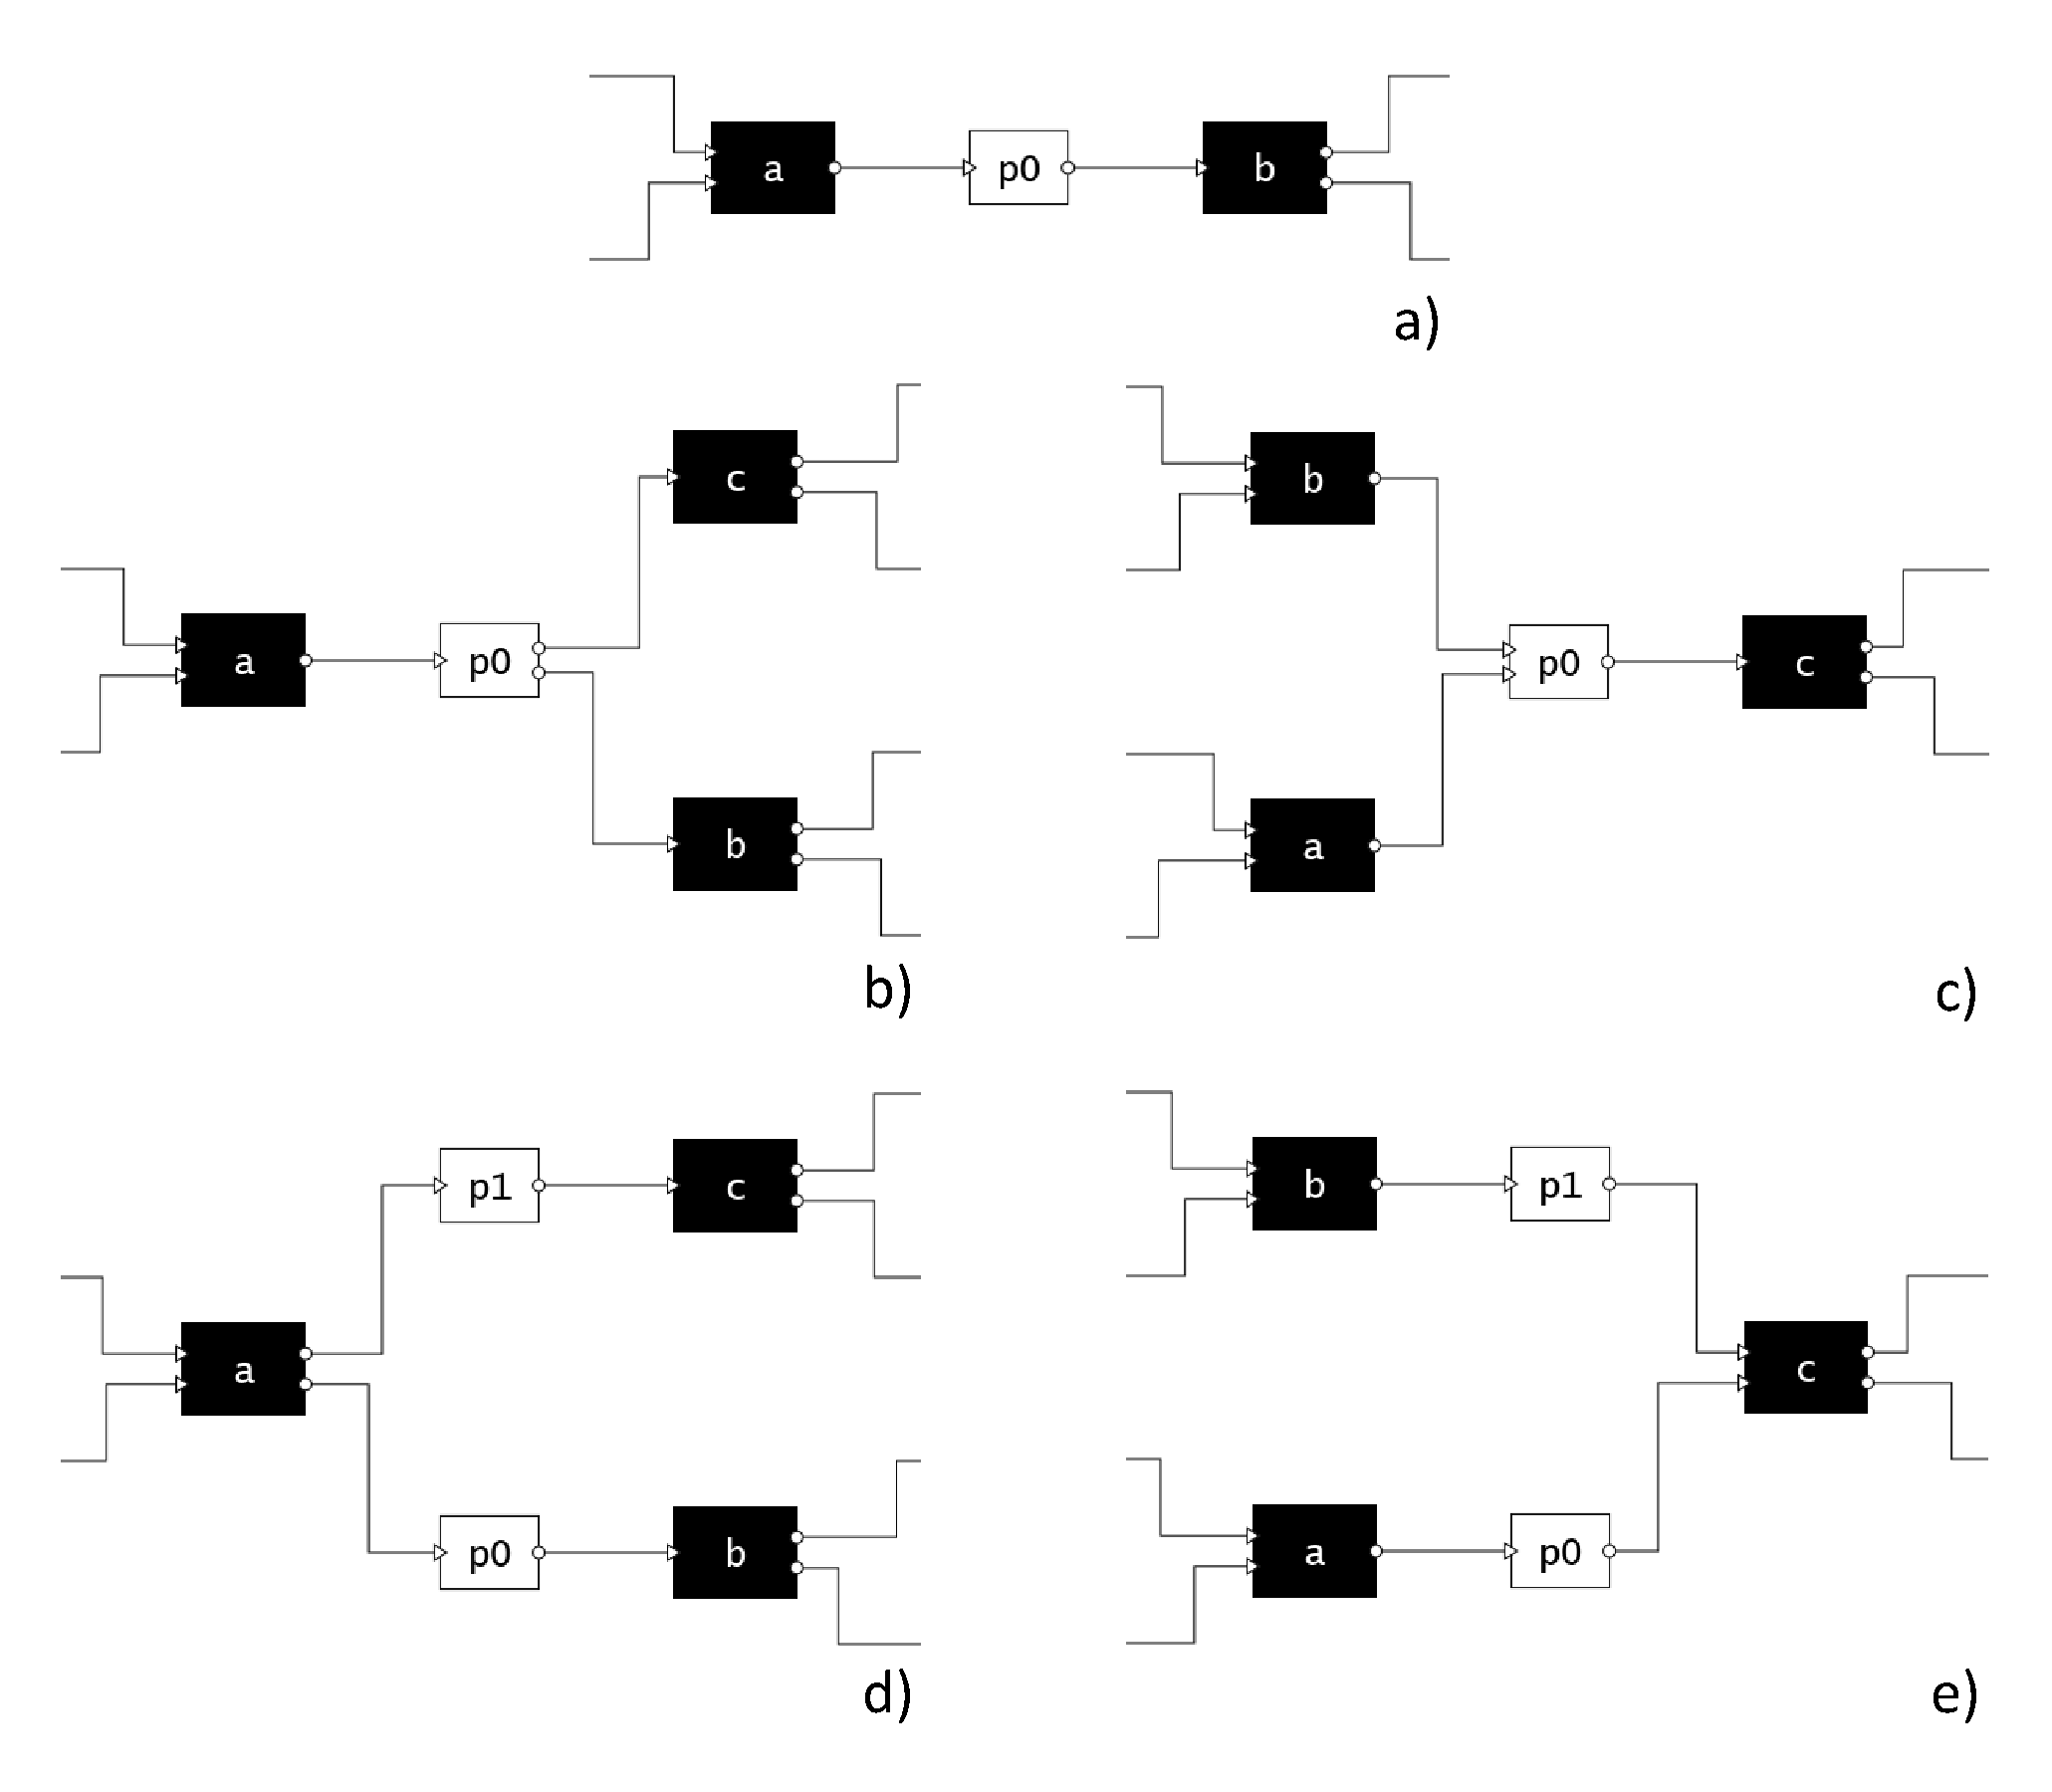
\includegraphics[width=0.8\textwidth]{pics/wfn-patterns.pdf}
\captionstyle{normal}\caption{Process patterns in WFN model. a) Sequence, b) XOR-split, c) XOR-join,\\d) AND-split, e) AND-join.}
\label{fig:wfn-patterns}
\end{figure}

Рассмотрим основные локальные шаблоны протекания процесса, которые можно отобразить с помощью WFN (см. рисунок~\ref{fig:wfn-patterns}).

На рисунке~\ref{fig:wfn-patterns} a) представлена обычная последовательность активностей $a \rightarrow b$.
Данный шаблон предписывает, что после выполнения активности $a$ токен будет помещен в место $p0$.
После этого окажется, что для активности $b$ выполнено условие, что все ее предшественники содержат токены (так как единственный предшественник $b$ это $p0$).
Таким образом, активность $b$ будет выполнена, токен удален из места $p0$ и новые токены будут отправлены по выходным дугам в узлы-последователи активности $b$.
     
На рисунке~\ref{fig:wfn-patterns} b) показан шаблон XOR-split, который реализует выбор одной из активностей после выполнения активности $a$.
После выполнения активности $a$ место $p0$ оказывается занятым токеном, который может быть использован при выполнении только одной из активностей $b$ или $c$.
Таким образом возможно выполнение либо последовательности активностей $a \rightarrow b$, либо последовательности $a \rightarrow c$.

На рисунке~\ref{fig:wfn-patterns} c) показан шаблон XOR-join, который по аналогии реализует выполнение либо последовательности активностей $a \rightarrow c$, либо последовательности активностей $a \rightarrow b$.

На рисунке~\ref{fig:wfn-patterns} d) показан шаблон AND-split, который реализует выполнение обеих активностей $b$ и $c$ после выполнения активности $a$.
Как только активность $a$ оказывается выполненной, то в места $p0$ и $p1$ попадают токены, которые делают возможным выполнение активностей $b$ и $c$.
При этом не важен порядок, в котором эти активности будут выполнены.

На рисунке~\ref{fig:wfn-patterns} e) показан шаблон AND-join, демонстрирующий, каким образом активность $c$ может быть выполнена только после выполнения обеих активностей $a$ и $b$.
Активность $c$ требует для своего выполнения наличия токенов сразу в $p0$ и $p1$, а это может произойти только после выполнения обеих активностей $a$ и $b$.

После описания данной упрощенной модели процесса с помощью WFN можно перейти собственно к алгоритму построения модели на основании журнала событий.
В данном случае журналом событий является просто список сценариев, каждый из которых представляет собой упорядоченную последовательность активностей.
Требуется по предоставленному журналу событий построить модель процесса, описанную с помощью WFN, которая реализует все сценарии из данного журнала.

Будем рассматривать простые сценарии, на которых будет видно, насколько сильно влияют записи журнала событий на реальную модель процесса.
Например, пусть у нас есть идеальная модель некоторого процесса, который состоит из фиксированной последовательности активностей, которые должны быть выполнены в строго определенной последовательности.
Вот эта последовательность активностей: $a \rightarrow b \rightarrow c \rightarrow d \rightarrow e \rightarrow f$.
Данной последовательности активностей соответствует следующая модель процесса, представленная на рисунке~\ref{fig:origin1}

\begin{figure}[h]
\setcaptionmargin{5mm}
%\onelinecaptionsfalse % if the caption is multiline
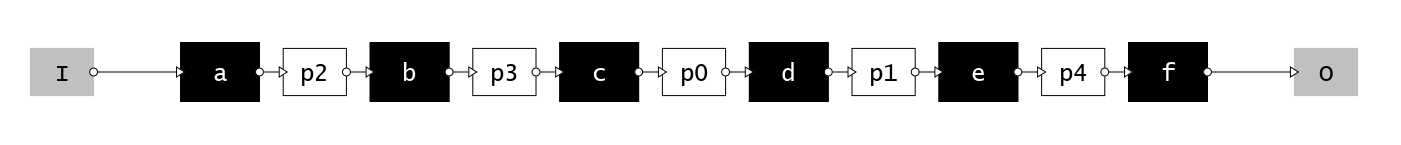
\includegraphics[width=0.95\textwidth]{pics/origin1.png}
\captionstyle{normal}\caption{Модель процесса, построенная по одному сценарию $a \rightarrow b \rightarrow c \rightarrow d \rightarrow e \rightarrow f$.}
\label{fig:origin1}
\end{figure}

Даже если все участники процесса согласны с такой определенной последовательностью активностей, которая необходима для протекания сценария, то обычно в реальности случаются ситуации, когда процесс протекает по-другому.
Представим себе простую ситуацию, когда ввиду спешки или форс-мажора были опущены все промежуточные активности в выполнении сценария и в журнале событий оказалась запись $a \rightarrow f$.
На рисунке~\ref{fig:second1} показана новая модель процесса, которая отражает также и этот появившийся упрощенный сценарий.

\begin{figure}[h]
\setcaptionmargin{5mm}
%\onelinecaptionsfalse % if the caption is multiline
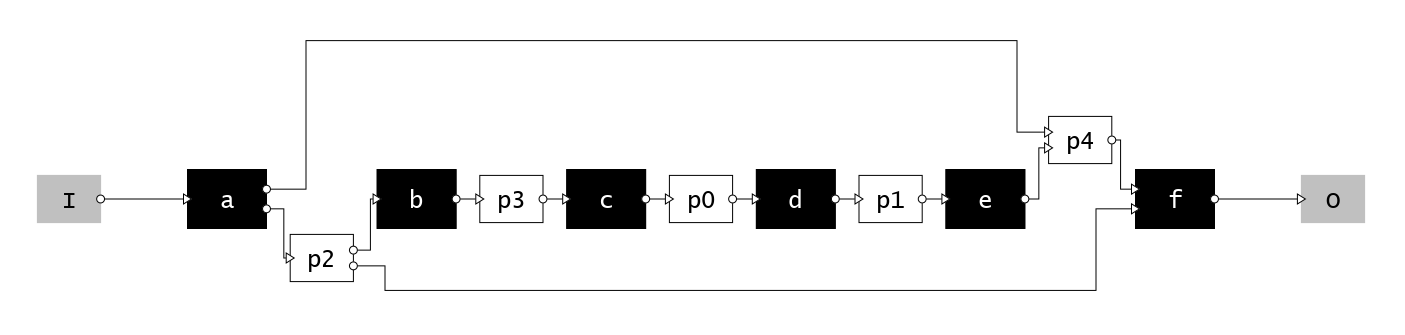
\includegraphics[width=0.95\textwidth]{pics/second1.png}
\captionstyle{normal}\caption{Скорректированная модель процесса после обработки сценария $a \rightarrow f$.}
\label{fig:second1}
\end{figure}

На этом рисунке мы уже видим появление шаблонов XOR-split и XOR-join, и в общем модель процесса заметно усложнилась.

А теперь рассмотрим еще более расширенный журнал событий, в котором попадаются сценарии с другими отклонениями.
В частности рассмотрим сценарий с нарушением порядка выполнения активностей, оборванный сценарий и сценарий с повторным выполнением некоторых последовательностей активностей.
Соберем полный журнал событий, он будет иметь следующий вид:

\begin{eqnarray*}
a \rightarrow b \rightarrow c \rightarrow d \rightarrow e \rightarrow f \\
a \rightarrow f \\
a \rightarrow b \rightarrow d \rightarrow c \rightarrow e \rightarrow f \\
a \rightarrow b \rightarrow c \\
a \rightarrow b \rightarrow c \rightarrow d \rightarrow e \rightarrow b \rightarrow c \rightarrow d \rightarrow e \rightarrow f
\end{eqnarray*}

При построении модели процесса по представленному журналу событий, мы получим схему, изображенную на рисунке~\ref{fig:third1}.

\begin{figure}[h]
\setcaptionmargin{5mm}
%\onelinecaptionsfalse % if the caption is multiline
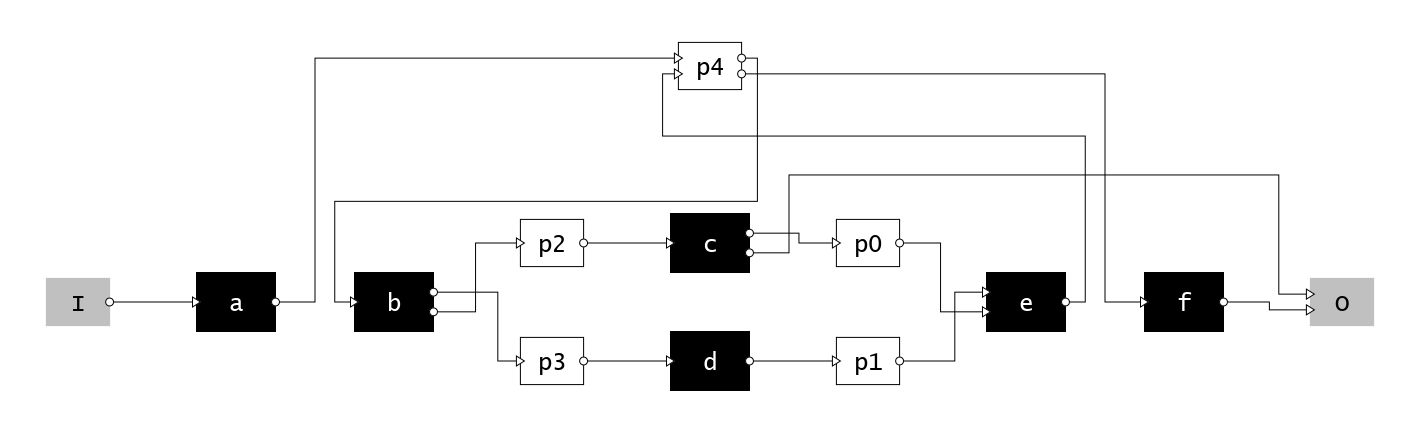
\includegraphics[width=0.95\textwidth]{pics/third1.png}
\captionstyle{normal}\caption{Модель процесса, построенная по журналу событий, содержащему сценарии с искажениями.}
\label{fig:third1}
\end{figure}

Данная модель процесса, конечно, не имеет ничего общего с идеальной моделью с рисунка~\ref{fig:origin1}.
Так же очевидно, что любой анализ следует проводить с использованием этой реальной модели, а не идеальной.
Построение же реальной модели по журналу событий может быть выполнено только автоматически, так как любые искажения реальных сценариев существенно влияют на топологию модели.
Заметим также, что в приведенных примерах показаны совершенно тривиальные сценарии, которые и близко не подходят к сложностям реально протекающих бизнес-процессов.
Поэтому для построения моделей реальных процессов для настоящих журналов событий требуются эффективные алгоритмы.

Опишем простейший алгоритм конструирования модели процесса по журналу событий.
В процессе описания алгоритма будем сразу же показывать его работу на уже рассмотренном модельном журнале событий (обозначим его $L$).

Итак, пусть у нас есть журнал событий

\begin{equation}
\begin{aligned}
L = [
&{a \rightarrow b \rightarrow c \rightarrow d \rightarrow e \rightarrow f},\\
&{a \rightarrow f},\\
&{a \rightarrow b \rightarrow d \rightarrow c \rightarrow e \rightarrow f},\\
&{a \rightarrow b \rightarrow c},\\
&{a \rightarrow b \rightarrow c \rightarrow d \rightarrow e \rightarrow b \rightarrow c \rightarrow d \rightarrow e \rightarrow f}
]
\end{aligned}
\end{equation}

Сначала нужно определить множество всех активностей, присутствующих журнале событий ($A$).
Кроме того, нужно определить множество активностей, с которых начинаются сценарии из журнала событий ($A_I \subset A$), а также активностей, которыми заканчиваются сценарии из журнала событий ($A_O \subset A$).

\begin{equation}
\begin{aligned}
&A = \{a, b, c, d, e, f\} \\
&A_I = \{a\} \\
&A_O = \{c, f\}
\end{aligned}
\end{equation}

Для следующего шага требуется построение матрицы последовательностей активностей ($M_S$).
Данная матрица является квадратной, она имеет размер равный общему количеству активностей, и ее элемент $M_S[x, y]$ содержит единицу, если в журнале событий найдется сценарий, в котором встречается последовательность $x \rightarrow y$.

Матрица $M_S$ для нашего тестового журнала событий выглядит следующим образом:

\begin{equation}
M_S = \begin{vmatrix}
\ & [a] & [b] & [c] & [d] & [e] & [f] \\
[a] & 0 & 1 & 0 & 0 & 0 & 1 \\ 
[b] & 0 & 0 & 1 & 1 & 0 & 0 \\
[c] & 0 & 0 & 0 & 1 & 1 & 0 \\
[d] & 0 & 0 & 1 & 0 & 1 & 0 \\
[e] & 0 & 1 & 0 & 0 & 0 & 1 \\
[f] & 0 & 0 & 0 & 0 & 0 & 0
\end{vmatrix}
\end{equation}

Далее строится матрица отношений $M_R$.
Она имеет такой же размер, что и матрица $M_S$, и ее элементы определяют отношения между активностями, которые должны быть отражены в построенной модели процесса.
Отношение строгого следования между активностями $x$ и $y$ (будем обозначать его через $x \Rightarrow y$) означает, что в журнале событий найдется сценарий, в котором $x \rightarrow y$, но не найдется такого сценария, в котором $y \rightarrow x$.
Другими словами, активности $x$ и $y$ связаны отношением жесткого следования, если $M_S[x, y](1 - M_S[y, x]) = 1$.
Аналогично, активности $x$ и $y$ можно назвать параллельными, если в некоторых сценариях за $x$ может следовать $y$, а в других сценариях за $y$ может следовать $x$.
Условием параллельности активностей является условие $M_S[x, y]M_S[y, x] = 1$ (обозначение $x \ || \ y$).
Если же ни в каких сценариях не обнаружено последовательностей $x \rightarrow y$ или $y \rightarrow x$, то отношение между такими актвностями будем называть неопределенностью.
Условие неопределенности -- $(1 - M_S[x, y])(1 - M_S[y, x]) = 1$ (обозначение $x \ ? \ y$).

Для рассматриваемого журнала событий матрица $M_R$ выглядит следующим образом:

\begin{equation}\label{eqn:r}
M_R = \begin{vmatrix}
\ & [a] & [b] & [c] & [d] & [e] & [f] \\
[a] & ? & \Rightarrow & ? & ? & ? & \Rightarrow \\ 
[b] & \Leftarrow & ? & \Rightarrow & \Rightarrow & \Leftarrow & ? \\
[c] & ? & \Leftarrow & ? & || & \Rightarrow & ? \\
[d] & ? & \Leftarrow & || & ? & \Rightarrow & ? \\
[e] & ? & \Rightarrow & \Leftarrow & \Leftarrow & ? & \Rightarrow \\
[f] & \Leftarrow & ? & ? & ? & \Leftarrow & ?
\end{vmatrix}
\end{equation}

После построения матрицы отношений между активностями можно перейти к построению множества мест для токенов в модели процесса ($P$).
Место для токена должно быть построено для каждой такой пары непересекающихся подмножеств активностей $X \subset A$, $Y \subset A$, что выполнено два условия.
Во-первых, любые две активности из $X$ связаны соотношением неопределенности, также любые две активности из $Y$ связаны соотношением неопределенности.
Во-вторых, любая активность $x \in X$ связана с любой активностью $y \in Y$ соотношением $x \Rightarrow y$. 
В этом случае строится место токена $p(X, Y)$, его узлами-предшественниками становятся все активности из $X$, а узлами-последователями -- все активности из $Y$.

В нашем рассматриваемом случае множество мест токенов выглядит следующим образом:

\begin{equation}
\begin{aligned}
P = \{
& p(\{d\}, \{e\}),
p(\{c\}, \{e\}),
p(\{e\}, \{f\}),
p(\{e\}, \{b\}),
p(\{e\}, \{f, b\}), \\
& p(\{a\}, \{f\}),
p(\{a\}, \{b\}),
p(\{a\}, \{f, b\}),
p(\{e, a\}, \{f\}),
p(\{e, a\}, \{b\}), \\
& p(\{e, a\}, \{f, b\}),
p(\{b\}, \{d\}),
p(\{b\}, \{c\})
\}
\end{aligned}
\end{equation}

Финальным шагом в формировании WFN, который представляет модель процесса, является удаление лишних мест токенов.
Если в наборе мест токенов найдутся два места $p(X, Y) \in P$ и $p(X', Y') \in P$ такие, что $X' \subseteq X$ и $Y' \subseteq Y$, то место $p(X', Y')$ является избыточным, и его можно удалить из модели.

После удаления избыточных мест, финальное множество место токенов примет свой окончательный вид:

\begin{equation}
\begin{aligned}
P = \{
p(\{d\}, \{e\}), p(\{c\}, \{e\}), p(\{e, a\}, \{f, b\}), p(\{b\}, \{d\}), p(\{b\}, \{c\})
\}
\end{aligned}
\end{equation}

Набор приведенных мест токенов приводит нас к модели процесса, изображенной на рисунке~\ref{fig:third1}.

\section{Simple Process Discovery Algorithm Optimization}

В приведенном в предыдущем разделе алгоритме узким местом является конструирование множества мест токенов $P$ с последующим удалением избыточностей.
При возрастании количества сценариев в журнале событий и общего количества активностей количество возможных комбинаций подмножеств активностей для формирования мест токенов растет экспоненциально.
При этом большая часть построенных токенов впоследствии все равно должна быть удалена, так как при построении будет много избыточных мест.
Например, при построенном месте $p(\{a, b\}, \{c, d\})$ в множество $P$ обязательно попадут следующие избыточные места: $p(\{a\}, \{c\})$, $p(\{a\}, \{d\})$, $p(\{b\}, \{c\})$, $p(\{b\}, \{d\})$.
В дальнейшем эти избыточные места будут удалены.
Поэтому требуется подход по построению множества мест токенов $P$, в котором избыточные места отсутствуют с самого начала.

\begin{figure}[h]
\setcaptionmargin{5mm}
%\onelinecaptionsfalse % if the caption is multiline
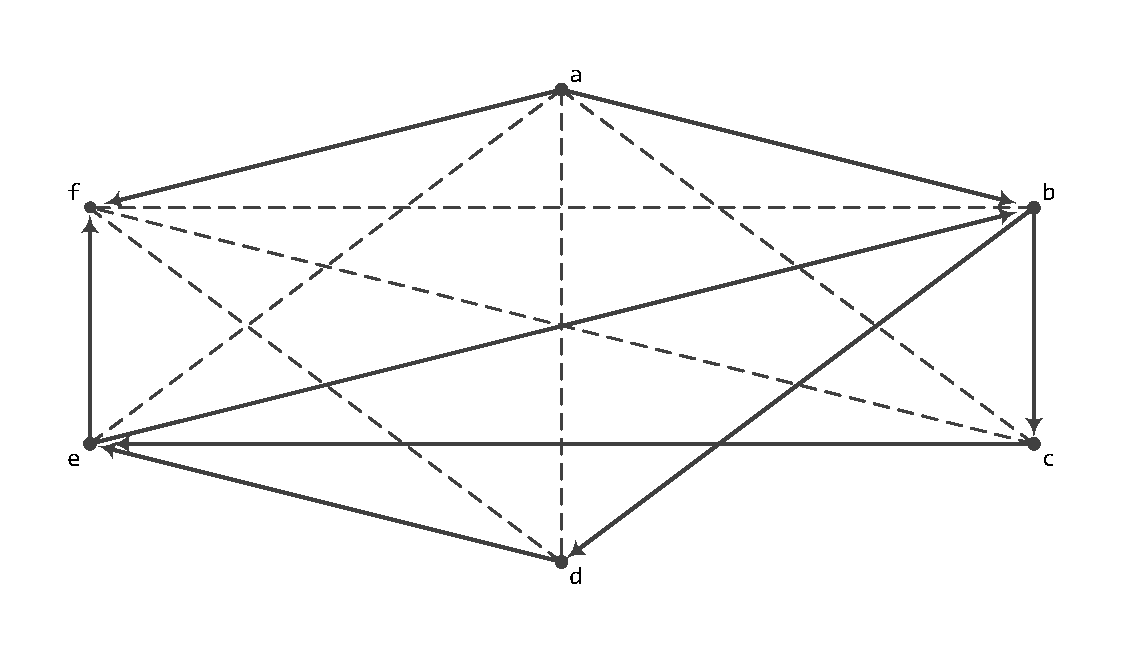
\includegraphics[width=0.8\textwidth]{pics/g_r.pdf}
\captionstyle{normal}\caption{Граф отношение $G_R$. Направленные ребра иллюстрируют отношения строгого следования, пунктирные ненаправленные ребра показывают отношением неопределенности.}
\label{fig:g_r}
\end{figure}

Множество мест токенов без избыточностей может быт построено на основе графа отношений между активностями.
Рассмотрим еще раз матрицу отношений $M_R$ из (\ref{eqn:r}).
В ней нам потребуются только отношения жесткого следования и неопределенности.
Построим вспомогательный граф отношений ($G_R$), узлами которого являются активности.
Далее, рассматриваемый граф содержит ребра двух видов.
Направленные ребра будут отображать отношения жесткого следования (два узла $x$ и $y$ соединены направленным ребром, если $x \Rightarrow y$).
Также в графе будут ненаправленные ребра, соединяющие узлы, связанные отношением неопределенности.
Для нашего рассматриваемого тестового примера граф отношений приведен на рисунке~\ref{fig:g_r}.

После формирования графа отношений $G_R$ нужно провести его стягивание по пунктирным ребрам (которые соответствуют отношению неопределенности).
За один шаг выполняется стягивание по одному ребру по следующим правилам.
Если в графе $G_R$ существует пара активностей $x$, $y$, связанных отношением $x \ ? \ y$, то можно выполнить стягивание по этому ребру.
При этом нужно осуществлять коррекцию отношений с другими активностями графа.
Если в графе есть активность $z$ такая, что $z \Rightarrow x$, $z \Rightarrow y$, то эти отношения удаляются, а вместо них добавляется отношение $z \Rightarrow xy$.
Если в графе есть активность $z$ такая, что $x \Rightarrow z$, $y \Rightarrow z$, то эти отношения удаляются, а вместо них добавляется отношение $xy \Rightarrow z$.
Если в графе есть активность $z$ такая, что $z \ ? \ x$, $z \ ? \ y$, то следует добавить также отношение $z \ ? \ xy$.

\begin{figure}[h]
\setcaptionmargin{5mm}
%\onelinecaptionsfalse % if the caption is multiline
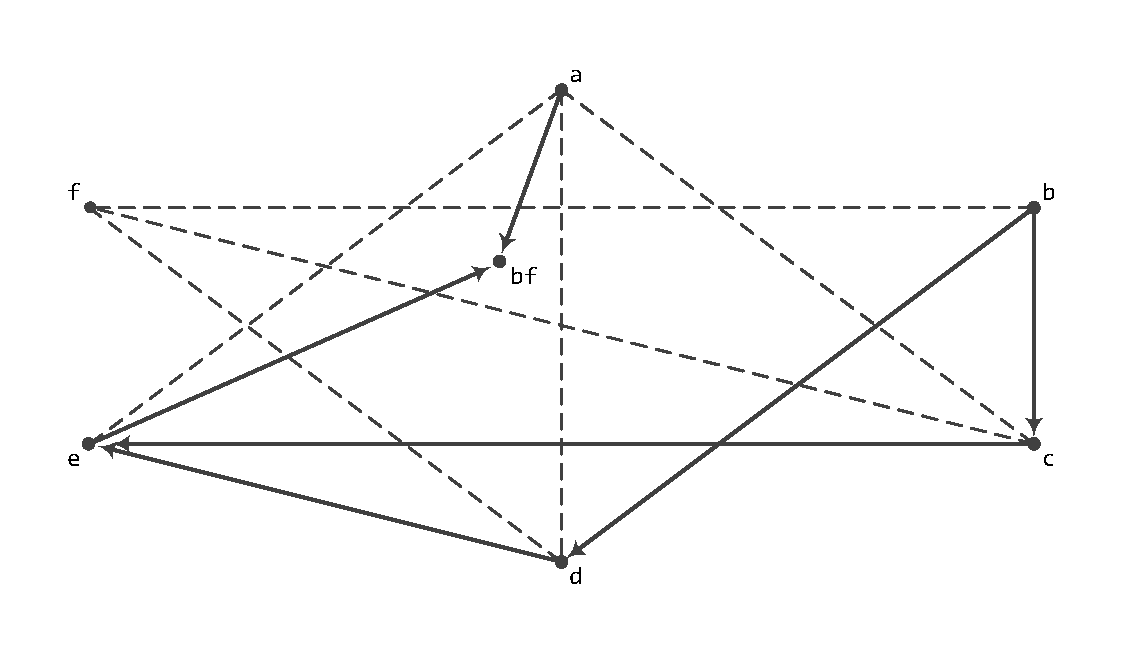
\includegraphics[width=0.8\textwidth]{pics/g_r_reduce1.pdf}
\captionstyle{normal}\caption{Редуцирование графа отношенией активностей. Шаг 1.}
\label{fig:g_r_reduce1}
\end{figure}

\begin{figure}[h]
\setcaptionmargin{5mm}
%\onelinecaptionsfalse % if the caption is multiline
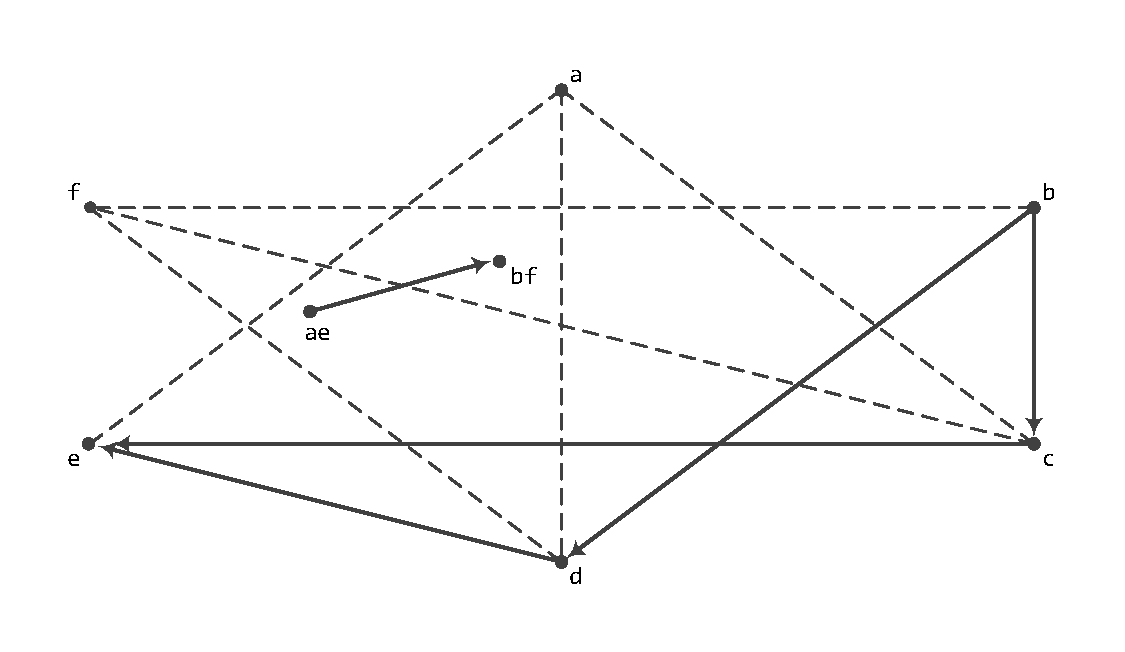
\includegraphics[width=0.8\textwidth]{pics/g_r_reduce2.pdf}
\captionstyle{normal}\caption{Редуцирование графа отношенией активностей. Шаг 2.}
\label{fig:g_r_reduce2}
\end{figure}

На рисунке~\ref{fig:g_r_reduce1} показан один шаг стягивания графа $G_R$ по ребру $b \ ? \ f$.
На рисунке~\ref{fig:g_r_reduce2} показан следующий шаг стягивания графа, уже по ребру $a \ ? \ e$.
Другие стягивания на данном графе выполнять не имеет смысла, после выполнения двух шагов граф содержит 5 направленных ребер, каждое из которых соответствует месту токена в модели процесса, показанной на рисунке~\ref{fig:third1}.

\section{Conclusion}

Conclusion.

\begin{acknowledgments}
The work has been done at the JSCC RAS as part of the state assignment for the topic ... The supercomputer MVS-10P, located at the JSCC RAS, was used for calculations during the research.
\end{acknowledgments}

\begin{thebibliography}{99}

\bibitem{Rettinger}
\refitem{article}
C. Rettinger, C. Godenschwager, S. Eibl, et al., {\it ``Fully Resolved Simulations of Dune Formation in Riverbeds"}, ISC High Performance , LNCS~{\bf 10266}, 3--21 (2017).

\end{thebibliography}

\end{document}
